% #####################################################################
% #####################################################################
% ##                                                                 ##
% ##                             Lizenz:                             ##
% ##                         CC BY-NC-SA 3.0                         ##
% ##      http://creativecommons.org/licenses/by-nc-sa/3.0/de/       ##
% ##                                                                 ##
% #####################################################################
% ##   Diese Datei kann beliebig verändert werden, solange darauf    ##
% ##     hingewiesen wird, dass dieses Dokument ursprünglich von     ##
% ##                                                                 ##
% ##                        www.ei-studium.de                        ##
% ##                                                                 ##
% ##                             stammt.                             ##
% ## Dies gilt insbesondere auch für alle daraus erstellten Dateien. ##
% ##    Des Weiteren muss die Weitergabe dieser Dateien unter der    ##
% ##                    gleichen Lizenz erfolgen.                    ##
% #####################################################################
% #####################################################################
\documentclass[a4paper,twocolumn,10pt]{article}
\usepackage[utf8]{inputenc}
\usepackage[ngerman]{babel}
\usepackage[top=2.0cm,bottom=1.5cm,left=1.0cm,right=1.0cm]{geometry}
\usepackage{enumitem}
\usepackage{graphicx}
\usepackage{amsfonts}
\usepackage{amsmath}
\usepackage{sectsty}
\usepackage{colortbl}
\usepackage{cancel}
\usepackage{listings}
\usepackage{color}
\usepackage{amsmath}
\usepackage{amssymb}
\usepackage{trsym}
\usepackage{scalefnt}
\usepackage{sectsty}
\usepackage{multirow}
\usepackage{ifthen}
\usepackage{mathrsfs}
\usepackage{fancyhdr}
\usepackage[pdfborder={0 0 0}]{hyperref}

\setlist{itemsep=.01mm}
\setenumerate{label=\emph{\arabic*})}
\setlength{\columnsep}{1cm}
\parindent 0mm

\partfont{\huge}
\sectionfont{\large \sc\bf}
\subsectionfont{\normalsize}
\subsubsectionfont{\small\textit}

\pagestyle{fancy}
\lhead[\leftmark]{Formelsammlung Stochastische Signale}
\chead[\leftmark]{\url{http://www.ei-studium.de}}
\rhead[\leftmark]{Erstelldatum: \today}
\lfoot[\leftmark]{Keine Garantie auf Vollständigkeit und Richtigkeit!}
\cfoot[\leftmark]{}
\rfoot[\leftmark]{\thepage}
\renewcommand{\headrulewidth}{0.5pt}
\renewcommand{\footrulewidth}{0.5pt}

\newcommand{\sollsein}{\stackrel{!}{=}}
\DeclareMathOperator{\cov}{cov}
\DeclareMathOperator{\str}{str}
\DeclareMathOperator{\val}{val}

\newenvironment{abc}{\begin{enumerate}[label={\alph*)}]}{\end{enumerate}}
\newenvironment{iii}{\begin{enumerate}[label={\roman{*})}]}{\end{enumerate}}
\newcommand{\var}{\mathsf{Var}}
\newcommand{\varX}{\mathsf{Var[X]}}
\newcommand{\erw}{\mathsf{E}}
\newcommand{\erwX}{\mathsf{E[X]}}
\newcommand{\e}{\mathsf{e}}
\renewcommand{\exp}{\mathsf{exp}}
\newcommand{\X}{\mathsf{X}}
\newcommand{\im}{\mathrm{j}}
\newcommand{\fa}{\TransformHoriz}
\newcommand{\fs}{\InversTransformHoriz}

\begin{document}
{\small \tableofcontents}
\newpage

\part{Wahrscheinlichkeitstheorie}

\section{Wahrscheinlichkeitsräume}
Ein \textbf{Wahrscheinlichkeitsraum} besteht aus einem Tripel $(\Omega ,\mathbb{F} ,P)$.

\subsection{Ergebnismenge $\Omega$}
Die nichtleere Menge $\Omega$ aller relevanten Ergebnisse eines Experiments heißt \textbf{Ergebnismenge}.

\subsection{Ereignisalgebra $\mathbb F$}
Das Mengensystem $\mathbb F \subseteq \mathbb P(\Omega)$ (Potenzmenge von $\Omega$) wird als \textbf{Ergebnisalgebra} bezeichnet, wenn es folgende Bedingungen erfüllt:
\begin{iii}
\item $\Omega \in \mathbb F$
\item $A \in \mathbb F \Rightarrow A^c \in \mathbb F$
\item $A_1,\dots,A_k \in \mathbb F \Rightarrow \bigcup_{i=1}^k A_i \in \mathbb F$
\end{iii}
Daraus folgt weiterhin:
\begin{iii}
\item $\emptyset \in \mathbb F$
\item $A_i \backslash A_j \in \mathbb F$
\item $\bigcap_{i=1}^k A_i \in \mathbb F$
\end{iii}
Das Mengensystem $\mathbb F$  wird als \textbf{$\sigma$-Algebra} bezeichnet, falls $k\rightarrow\infty$ und obige Bedingungen erfüllt sind.\\\\
Das Tupel $(\Omega, \mathbb F)$ heißt \textbf{Ereignisraum} oder \textbf{messbarer Raum}.

\subsection{Wahrscheinlichkeitsmaß P}
\begin{iii}
\item $P(A) \geq 0$
\item $P(\Omega) = 1$
\item $P(\bigcup_{i=1}^\infty A_i) = \sum_{i=1}^\infty P(A_i)$, wenn $A_i \cap A_j = \emptyset, \forall i \neq j$
\end{iii}
Weitere Eigenschaften von $P$:
\begin{iii}
\item $P(A^c) = 1 - P(A)$
\item $P(\emptyset) = 0$
\item $P(A \backslash B) = P(A \cap B^c) = P(A) - P(A \cap B)$
\item $P(A \cup B) = P(A) + P (B) - P(A \cap B)$
\item $A \subset B \Rightarrow P(A) \leq P(B)$
\item $P(\bigcup_{i=1}^k A_i) \leq \sum_{i=1}^k P(A_i)$
\end{iii}

\section{Bedingte Wahrscheinlichkeit und stochastische Unabhängigkeit}
\subsection{Bedingte Wahrscheinlichkeit}
\[P(B \mid A) \triangleq P_A(B) = \frac{P(A \cap B)}{P(A)}\]
\[\Rightarrow P(A \cap B) = P(A \mid B)P(B) = P(B \mid A)P(A) \]

\subsubsection{Gesetz der totalen Wahrscheinlichkeit}
$B_i$ sei eine Zerlegung von $\Omega$, dann gilt:
\[P(A) = \sum_{i \in I} P(A \mid B_i)P(B_i)\]

\subsubsection{Satz von Bayes}
\[P(B_j \mid A) = \frac{P(A \mid B_j)P(B_j)}{\sum_{i \in I} P(A \mid B_i)P(B_i)}=\frac{P(A\cap B_j)}{P(A)}\]

\subsubsection{Multiplikationssatz}
\[P(A\cap B\cap C\cap D)=P(A|B\cap C\cap D)P(B|C\cap D)P(C|D)P(D) \]

\subsection{Stochastische Unabhängigkeit}
Zwei Ereignisse $A$ und $B$ sind dann von einander unabhängig, wenn gilt: \[P(A \cap B) = P(A)P(B) \]
Dann gilt auch: \[P(B \mid A) = P(B) \]
Für jede endliche Teilmenge $\emptyset \neq J\subset I$ gilt dann:
 \[(\bigcap_{i \in I} A_i) = \prod_{i \in I} P(A_i) \]

\section{Zufallsvariablen und Wahrscheinlichkeitsverteilung}

\subsection{Zufallsvariablen}
$\mathsf X : \Omega \rightarrow \Omega'$ heißt Zufallsvariable, wenn für jedes $A' \in \mathbb F'$ ein $A \in \mathbb F$ existiert mit $A = \{\omega \in \Omega \mid \mathsf X(\omega) \in A'\} \in \mathbb F$.
\begin{abc}
\item $\mathsf X : \Omega \rightarrow \mathbb R$ heißt \textbf{reelle Zufallsvariable}, wenn $\{\omega \in \Omega \mid \mathsf X(\omega) \leq x\} = \{\mathsf X \leq x \} \in \mathbb F\ \forall\ x \in \mathbb R$.
\item $\vec{\mathsf X} : \Omega \rightarrow \mathbb R^n, n \in \mathbb N$ heißt \textbf{mehrdimensionale (reelle) Zufallsvariable}, wenn $ \vec{\mathsf X} = [\mathsf X_1,\dots,\mathsf X_n]^T$.
\item $\mathsf X : \Omega \rightarrow \mathbb C$ heißt \textbf{komplexe Zufallsvariable}, wenn $\operatorname{Re}(\mathsf X)$ und $\operatorname{Im}(\mathsf X)$ reelle Zufallsvariablen sind.
\item Zufallsvariablen $\mathsf X : \Omega \rightarrow \Omega'$, die $\Omega$ auf endliche oder abzählbare Mengen $\Omega'$ abbilden, heißten \textbf{diskrete Zufallsvariablen}.
\end{abc}

\subsection{Verteilung einer Zufallsvariable}
$P_\mathsf{X}(A')  \triangleq P(\{\omega \in \Omega \mid \mathsf{X}(\omega) \in A'\}) = P(\{\mathsf{X} \in A'\})\ \forall\ A' \in \mathbb F'$ heißt \textbf{Verteilung} von $\mathsf{X}$.

\subsubsection{Zähldichte für diskrete Zufallsvariablen (PMF)}
\[p_\mathsf{X}(x) = P(\{\mathsf{X} = x \})\]

\subsubsection{Wahrscheinlichkeitsdichtefunktion (WDF)}
\[f_\mathsf{X}(x)=\frac{dF_\mathsf{X}(x)}{dx}\]
WDF einer \textbf{diskreten} Zufallsvariable $\X$:
\[f_\X(x)=\sum_{\xi\in\varOmega'}p_\X(\xi)\delta(x-\xi)\]

\subsubsection{Stetige kumulative Verteilungsfunktion (KMF)}
\[F_\mathsf{X}(x) = P(\{\mathsf{X} \leq x \})\]
\[F_\mathsf{X}(x) = \int_{-\infty}^{x} f_\mathsf{X}(\xi)\mathsf d\xi\]
\textbf{Eigenschaften:}
\begin{iii}
\item  $F_\mathsf{X}(x)$ ist monoten wachsend.
\item  $F_\mathsf{X}(x)$ ist rechsseitig stetig.
\item $\lim_{x \to -\infty}F_\mathsf{X}(x) = 0, \lim_{x \to \infty}F_\mathsf{X}(x) = 1$
\item  $P(\{a < \mathsf{X} \leq b \}) = F_\mathsf{X}(b) - F_\mathsf{X}(a)$
\item  $P(\{\mathsf{X} > c \}) = 1 - F_\mathsf{X}(c)$
\item $P({\X = x})= \begin{cases}
  p_\X(x) & \text{$\X$ ist reell und diskret}\\
  0 & \text{$\X$ ist stetig}
\end{cases}$   %evtl ändern%
\end{iii}

\subsubsection{Diskrete kumulative Verteilungsfunktion (KMF)}
\[F_\mathsf{X}(x) = \sum_{\xi \in \Omega' : \xi \leq x} p_\mathsf{X}(\xi)\]

\subsection{Mehrdimensionale Verteilungen}

\subsubsection{Gemeinsame Kumulative Verteilungsfunktion}
\[\begin{split}F_{\mathsf X_1,\dots,\mathsf X_n}(x_1,\dots,x_n) & =F_{\vec{\mathsf X}}(\vec x) = P(\{\vec{\mathsf X} \leq \vec x\})\\ & \triangleq P(\{\mathsf X_1 \leq x_1, \dots, \mathsf X_n \leq x_n\})\end{split}\]
\textbf{Eigenschaften:}
\begin{iii} 
\item $F_{\mathsf X_1,\dots,\mathsf X_n}$ ist in jeder Koordinate monoton wachsend.
\item $F_{\mathsf X_1,\dots,\mathsf X_n}$ ist im folgenden Sinn rechtsseitig stetig:  $\forall\ h > 0$ gilt $\lim_{h \to 0}F_{\mathsf X_1,\dots,\mathsf X_n}(x_1 + h,\dots,x_n + h) = F_{\mathsf X_1,\dots,\mathsf X_n}(x_1,\dots,x_n),\ \forall\ (x_1,\dots,x_n) \in \mathbb R^n$
\item Für jedes $1 \leq u \leq n$ gilt:\\ $\lim_{x_i \to -\infty}F_{\mathsf X_1,\dots,\mathsf X_n}(x_1,\dots,x_n) = 0$\\$\lim_{x_i \to \infty}F_{\mathsf X_1,\dots,\mathsf X_n}(x_1,\dots,x_n) = 1$
\end{iii}

\subsubsection {Verbund-Zähldichte}
\[\begin{split}p_{\mathsf X_1,\dots,\mathsf X_n}(x_1,\dots,x_n) &=p_{\vec{\mathsf X}}(\vec x) = P(\{\vec{\mathsf X} = \vec x\})\\ &\triangleq P(\{\mathsf X_1 = x_1, \dots, \mathsf X_n = x_n\})\end{split}\]

\subsubsection{Verbund-Wahrscheinlichkeitsdichtefunktion}
\[f_{\mathsf X_1,\dots,\mathsf X_n}(x_1,\dots,x_n) = \frac{\partial^nF_{\mathsf X_1,\dots,\mathsf X_n}(x_1,\dots,x_n)}{\partial x_1\dots\partial x_n}\]

\subsubsection{Stetige kumulative Verteilungsfunktion}
\begin{gather*}
F_{\mathsf X_1,\dots,\mathsf X_n}(x_1,\dots,x_n) \\ =\int_{-\infty}^{x_1}\dots\int_{-\infty}^{x_n}f_{\mathsf X_1,\dots,\mathsf X_n}(\xi_1,\dots,\xi_n)\mathsf d\xi_n\dots\mathsf d\xi_1\end{gather*}


\subsubsection{Marginalisierung / Randverteilungen}
Für $m < n$ gilt:
\[F_{\mathsf X_1,\dots,\mathsf X_m}(x_1,\dots,x_m)=F_{\mathsf X_1,\dots,\mathsf X_n}(x_1,\dots,x_m,\infty,\dots,\infty)\]
Es gilt:
\begin{abc}
\item Eine durch Marginalisierung auf eine einzige Zufallsvariable entstehende KVF heißt \textbf{Randverteilung}:
\[\begin{split} F_{\mathsf X_1}(x_1) &=F_{\mathsf X_1,\dots,\mathsf X_n}(x_1,\infty,\dots,\infty)\end{split}\]

\item \textbf{Zähldichte} $p_{\mathsf X_1}$
\[p_{\mathsf X_1}(x_1) = \sum_{x_2,\dots,x_n}p_{\mathsf X_1,\dots,\mathsf X_n}(x_1,\dots,x_n)\]

\item \textbf{Wahrscheinlichkeitsdichtefunktion}  $f_{\mathsf X_1}$
\[f_{\mathsf X_1}(x_1) = \int_{-\infty}^{\infty}\dots\int_{-\infty}^{\infty}f_{\mathsf X_1,\dots,\mathsf X_n}(x_1,\dots,x_n)\mathsf dx_n\dots\mathsf dx_2\]
\end{abc}

\subsection{Unabhängigkeit von Zufallsvariablen}
$\mathsf X_1,\dots,\mathsf X_n$ reelle Zufallsvariablen sind genau dann \textbf{stochastisch unabhängig} wenn für jedes $\vec x = [x_1,\dots,x_n]^T \in \mathbb R^n$ gilt: \[P(\{\mathsf X_1 \leq x_1,\dots,\mathsf X_n \leq x_n\}) = \prod_{i=1}^nP(\{\mathsf X_i \leq x_i\})\]Analog folgt die stochastische Unabhängigkeit 
\begin{abc}
\item für reelle Zufallsvariablen aus \[F_{\mathsf X_1,\dots,\mathsf X_n}(x_1,\dots,x_n) = \prod_{i=1}^nF_{\mathsf X_i}(x_i)\]
\item für reelle und diskrete Zufallsvariablen aus \[p_{\mathsf X_1,\dots,\mathsf X_n}(x_1,\dots,x_n) = \prod_{i=1}^np_{\mathsf X_i}(x_i)\]
\item für reelle und stetige Zufallsvariablen aus\[f_{\mathsf X_1,\dots,\mathsf X_n}(x_1,\dots,x_n) = \prod_{i=1}^nf_{\mathsf X_i}(x_i)\]
\end{abc}

\subsection{Bedingte Zufallsvariablen}

\subsubsection{Bedingte kumulative Verteilungsfunktion}
\[F_{\mathsf X \mid A}(x \mid A) = P_A(\{\mathsf X \leq x\}) = P(\{\mathsf X \leq x\} \mid A)\]

\subsubsection{Bedingte Zähldichte}
\[p_{\mathsf X \mid \mathsf Y}(x \mid y) = \frac{p_{\mathsf X, \mathsf Y}(x,y)}{p_\mathsf Y(y)}\]

\subsubsection{Bedingte Wahrscheinlichkeitsdichtefunktion}
\[f_{\mathsf X \mid \mathsf Y}(x \mid y) = \frac{\mathsf dF_{\mathsf X \mid \mathsf Y}(x \mid y)}{\mathsf dx} = \frac{f_{\mathsf X, \mathsf Y}(x,y)}{f_\mathsf Y(y)}\]

\section{Funktionen von Zufallsvariablen}

\subsection{Transformation von Zufallsvariablen (univariater Fall)}
Für eine beliebig differenzierbare Funktion $g$ gilt:
\[f_\mathsf Y(y) = \sum_{i=1}^{N}f_\mathsf X(x_i) \left[\left|\frac{\mathsf dg(x)}{\mathsf dx}\right|_{x=x_i}\right]^{-1}\]
\[f_\mathsf Y(y) = \sum_{i=1}^{N}f_\mathsf X(x_i)\left|\frac{\mathsf dx_i}{\mathsf dy}\right|\]
mit streng monotonen $x_i$:
\[x_i=g_i^{-1}(y)\]\\
\textbf{Beispiel:}\\
$Y=aX+b$ ($g(x)=ax+b$) mit $a\in\mathbb{R}\backslash 0,\;b\in\mathbb{R}$:
\[\Rightarrow f_Y(y)=\frac{1}{|a|}f_X\left(\frac{y-b}{a}\right)\]
\[F_Y(y)=\begin{cases}F_X\left(\frac{y-b}{a}\right) & a>0 \\ 1-F_X\left(\frac{y-b}{a}\right) & a<0\end{cases}\]

\subsection{Summe unabhängiger Zufallsvariablen}
Sei $\mathsf Z = \mathsf X + \mathsf Y$ ($\mathsf X$ und $\mathsf Y$ stoch. unabhängig), dann gilt
\[f_{\mathsf Z = \mathsf X + \mathsf Y}(z) = (f_\mathsf X * f_\mathsf Y)(z)=\int\limits_{-\infty}^{\infty}f_{\mathsf{X}}(z-y)f_{\mathsf{Y}}(y)dy\]

\section{Stochastische Standardmodelle}

\subsection {Diskrete Verteilungen}

\subsubsection{Diskrete Gleichverteilung}
\[p_\mathsf X(\omega) = \frac{1}{|\Omega|}, \omega \in \Omega\]

\subsubsection{Bernoulli-Verteilung}
\[p_\mathsf X(k) = \begin{cases}
  p  & \text{wenn }k = 1\\
  1-p & \text{wenn }k = 0\\
0 & \text{sonst}
\end{cases}\]
mit $0\leq p\leq 1$\\\\
\begin{tabular}{ll}
Erwartungswert: & $\erwX=p$\\
Varianz: &$\varX=p(1-p)$\\
Wahrscheinlichkeitserz. F.: &$G_\X(z)=pz+1-p$
\end{tabular}

\subsubsection{Binomialverteilung}
\[p_\mathsf X(k) = \binom n k p^k(1-p)^{n-k}\]
mit $ n \in \mathbb N;\;\;k \in \{ 0,1,\dots,n \};\;\;0\leq p\leq 1$\\
und $\binom{n}{k}=\frac{n!}{k!(n-k)!}$\\\\
\begin{tabular}{ll}
Erwartungswert: &$\erwX=np$\\
Varianz: &$\varX=np(1-p)$\\
Wahrscheinlichkeitserz. F.: &$G_\X(z)=(pz+1-p)^n$
\end{tabular}

\subsubsection{Poisson-Verteilung}
\[p_\mathsf X(k) = \frac{\lambda^k}{k!}\e^{-\lambda}\]
mit $\lambda \geq 0;\;\;k \in \mathbb N_0$\\\\
\begin{tabular}{ll}
Erwartungswert: &$\erwX=\lambda$\\
Varianz: &$\varX=\lambda$\\
Wahrscheinlichkeitserz. Funktion: &$G_\X(z)=\e^{\lambda(z-1)}$
\end{tabular}\\\\
Ergibt sich als asymptotischer Grenzfall aus der Binomialverteilung, wenn $n \rightarrow \infty$ und $p \rightarrow 0$, sodass $\lambda=np$:
\[p_\mathsf X(k) = \lim_{n \to \infty}B_{n,\frac{\lambda}{n}}(k)\]

\subsubsection{Geometrische Verteilung}
\[p_\mathsf X(k) = (1 - p)^{k-1}p\]
mit $0<p\leq 1;\;\;k \in \mathbb N$\\\\
\begin{tabular}{ll}
Erwartungswert: &$\erwX=\frac{1}{p}$\\
Varianz: &$\varX=\frac{1-p}{p^2}$\\
Wahrscheinlichkeitserz. Funktion: &$G_\X(z)=\frac{pz}{1-z+pz}$
\end{tabular}\\\\\\
Eine geometrisch verteilte ZV $\X$ ist \textbf{gedächtnislos}:
\[P(\{\mathsf X > n + k\} \mid \{\mathsf X > n\}) = P(\{\mathsf X > k\}),\; n,k \in \mathbb N_0\]

\subsection{Stetige Verteilungen}

\subsubsection{Gleichverteilung}
\[f_\X(x) =
\begin{cases}
  \frac{1}{b-a}  & a\leq x\leq b\\
  0 & \text{sonst}
\end{cases}\]
mit $ - \infty < a < b <\infty $\\\\
\begin{tabular}{ll}
Erwartungswert: &$\erwX=\frac{a+b}{2}$\\
Varianz: &$\varX=\frac{(b-a)^2}{12}$\\
Charakterist. Funktion: &$\varphi_\X(\omega)=\frac{\e^{\im\omega b} -\e^{\im\omega a}}{\im\omega(b-a)}$
\end{tabular}

\subsubsection{Exponentialverteilung}
\[f_\X(x) =\lambda \e^{-\lambda x}\]
mit $\lambda > 0;\;\;x \geq 0$\\\\
\begin{tabular}{ll}
Erwartungswert: &$\erwX=\frac{1}{\lambda}$\\
Varianz: &$\varX=\frac{1}{\lambda^2}$\\
Charakterist. Funktion: &$\varphi_\X(\omega)=\frac{\lambda}{\lambda-\im\omega}$
\end{tabular}\\\\\\
Eine exponentialverteilte ZV $\X$ ist \textbf{gedächtnislos}:
\[P(\{\mathsf X > x + \xi\} \mid \{\mathsf X > \xi\}) = P(\{\mathsf X > x\}),\, x, \xi \geq 0\]

\subsubsection{Normalverteilung}
\[f_\X(x) = \frac{1}{\sqrt{2\pi\sigma^2}}  \e^{-\frac{(x - \mu)^2}{2 \sigma^2}}\]
mit $\mu\in\mathbb{R};\;\;\sigma > 0$\\\\
\begin{tabular}{ll}
Erwartungswert: &$\erwX=\mu$\\
Varianz: &$\varX=\sigma^2$\\
Charakterist. Funktion: &$\varphi_\X(\omega)=e^{(\im\omega\mu-\frac{\omega^2\sigma^2}{2})}$
\end{tabular}\\\\
Für eine normalverteilte ZV $\mathsf X$ schreibt man auch
\[\mathsf X \sim \mathcal N(\mu, \sigma^2)\]
Für den Spezialfall $\mathsf X \sim \mathcal N(0, 1)$ spricht man von \textbf{Standardnormalverteilung}:
\[\phi(x)=\frac{1}{\sqrt{2\pi}}e^{-\frac{x^2}{2}}\]
Es gilt außerdem:
\begin{iii}
\item $\mathsf Y \sim \mathcal N(\mu, \sigma^2) \Rightarrow \mathsf X = \frac{1}{\sigma}(\mathsf Y-\mu) \sim \mathcal N(0, 1)$
\item $\mathsf X \sim \mathcal N(0, 1) \Rightarrow \mathsf Y = \sigma\mathsf X + \mu \sim \mathcal N(\mu, \sigma^2)$
\end{iii}
Für $X\sim\mathcal{N}(0,1)$ und $Y\sim\mathcal{N}(\mu,\sigma^2)$ gilt:
\[f_Y(y)=\frac{1}{\sigma}\phi\left(\frac{y-\mu}{\sigma}\right)\]
\[F_Y(y)=F_X\left(\frac{y-\mu}{\sigma}\right)\]
Sei $X\sim\mathcal{N}(\mu_X,\sigma_X^2)$ und $Y\sim\mathcal{N}(\mu_Y,\sigma_Y^2)$, dann gilt für $Z=X+Y$:
\[Z\sim\mathcal{N}(\mu_X+\mu_Y,\sigma_X^2+\sigma_Y^2)\]

\subsubsection{Multivariate Normalverteilung}
\[f_{\mathsf X_1,\dots,\mathsf X_n}(x_1,\dots,x_n)= \frac{1}{\sqrt{2\pi}^n\sqrt{\det(\mathbf C)}}e^{-\frac{1}{2}(\vec x - \vec \mu)^T\mathbf C^{-1}(\vec x - \vec \mu)}\]
wobei $\vec \mu$ den Erwartungswertvektor \[
\vec \mu = \begin{bmatrix} \mu_1\\\vdots \\\mu_n \end{bmatrix} =  \erw \begin{bmatrix} \mathsf X_1\\\vdots \\\mathsf X_n \end{bmatrix} = \erw[\vec{\mathsf X}]\] und $\mathbf C$ die Kovarianzmatrix \[\mathbf C = \erw[(\vec{\mathsf X} - \vec \mu)(\vec{\mathsf X} - \vec \mu)^T] = \mathbf C^T\] bezeichnet.\\
Analog zum univariaten Fall schreibt man auch \[\vec{\mathsf X} \sim \mathcal N(\vec \mu, \mathbf C)\]
Für $n$ paarweise unkorrelierte und gemeinsam normalverteilte Zufallsvariablen $X_1,...,X_2$ gilt:
\[C=diag[\sigma_1^2,...,\sigma_2^2]\]
\[f_{X_1,...,X_n}(x_1,...,x_n)=\prod\limits_{i=1}^{n}f_{X_i}(x_i)\]
$\Rightarrow X_1,...,X_2$ sind stochastisch unabhängig!

\section{Erwartungswert und Varianz}

\subsection{Erwartungswert diskreter reeller ZV}
\[\mu_{\mathsf{X}}=\erw[\mathsf X] = \sum_{x \in \Omega'}xP(\{\mathsf X = x\}) = \sum_{x \in \Omega'}xp_\mathsf X(x)\]
Sei $g: \mathbb R \rightarrow \mathbb R$ eine reellwertige Fkt. dann gilt für $\mathsf Y = g(\mathsf X)$ \[\erw[g(\mathsf X)] = \sum_{x \in \Omega'}g(x)p_\mathsf X(x)\]

\subsection{Erwartungswert stetiger Zufallsvariablen}
\[\erw[\mathsf X] = \int_{-\infty}^{\infty}xf_\mathsf X(x)\mathsf dx\]
Sei $g: \mathbb R \rightarrow \mathbb R$ eine reellwertige Fkt. dann gilt für $\mathsf Y = f(\mathsf X)$ \[\erw[g(\mathsf X)] = \int_{-\infty}^{\infty}g(x)f_\mathsf X(x)\mathsf dx\]

\subsection{Eigenschaften des Erwartungswerts}
Seien $\mathsf X$, $\mathsf Y$ reelle Zufallsvariablen, $\alpha, \beta \in \mathbb R$
\begin{iii}
\item $\erw[\alpha \mathsf X  + \beta \mathsf Y] = \alpha \erw[\mathsf X] + \beta \erw[\mathsf Y]$
\item $\mathsf X \leq \mathsf Y \Rightarrow \erw[\mathsf X] \leq \erw[\mathsf Y]$
\item $\mathsf X,Y$ stoch. unabhängig $\Rightarrow\erw[\mathsf X \mathsf Y] = \erw[\mathsf X]\erw[\mathsf Y]$\\
$E[XY]$ heißt \textbf{Korrelation} von $X,Y$
\item Falls $\mathsf X : \Omega \rightarrow \mathbb R_+$ (nur nichtnegative Werte):\\
\[\erw[\mathsf X] = \int\limits_{0}^{\infty} P(\mathsf X > t) \mathsf dt=\int\limits_{0}^{\infty}(1-F_{\mathsf{X}}(t))dt\]
\[\erw[\mathsf X] = \sum\limits_{k=0}^{\infty} P(\mathsf X > k)\]
\end{iii}

\subsection{Varianz und Kovarianz reeller Zufallsvariablen}
\[\sigma_{\mathsf{X}}^2=\var[\mathsf X] = \erw\left[(\mathsf X - \erw[\mathsf X])^2\right] = \erw[\mathsf X^2] - \erw[\mathsf X]^2\]
\[\begin{split}\text{Cov}[\mathsf X, \mathsf Y]&=\text{Cov}[\mathsf Y, \mathsf X] = \erw \left[ (\mathsf X - \erw[\mathsf X])(\mathsf Y - \erw[\mathsf Y])\right ] \\&= \erw[\mathsf X \mathsf Y] - \erw[\mathsf X]\erw[\mathsf Y]\end{split} \]

\subsection{Eigenschaften von Varianz und Kovarianz}
Seien $\mathsf X$, $\mathsf Y$, $\mathsf U$, $\mathsf V$ reelle Zufallsvariablen, $\alpha, \beta, \gamma, \delta \in \mathbb R$
\begin{iii}
\item $\var[\mathsf X] = \text{Cov}[\mathsf X, \mathsf X]$
\item $\text{Cov}[\alpha\mathsf X + \beta, \gamma\mathsf Y + \delta] = \alpha\gamma\text{Cov}[\mathsf X, \mathsf Y]$
\item $\text{Cov}[\mathsf X + \mathsf U, \mathsf Y + \mathsf V] \\= \text{Cov}[\mathsf X, \mathsf Y] + \text{Cov}[\mathsf X, \mathsf V] + \text{Cov}[\mathsf U, \mathsf Y] + \text{Cov}[\mathsf U, \mathsf V]$
\item $\var[\alpha\mathsf X + \beta] = \alpha^2\var[\mathsf X]$
\item $\var\left[\sum\limits_{i=1}^n\mathsf X_i\right] = \sum\limits_{i=1}^n\var[\mathsf X_i] + \sum\limits_{i=1}^n\sum\limits_{i \neq j}\text{Cov}[\mathsf X_i, \mathsf X_j]$
\item $\mathsf X$ und $\mathsf Y$ heißen \textbf{unkorreliert}, wenn\\$\text{Cov}[\mathsf X, \mathsf Y] = 0 \Leftrightarrow \erw[\mathsf X \mathsf Y] = \erw[\mathsf X]\erw[\mathsf Y]$
\item $\mathsf X,\mathsf Y$ sind \textbf{orthogonal} $\Leftrightarrow\erw[\mathsf X \mathsf Y] = 0$
\item Sind $\mathsf X_i, i \in \{1,\dots,n\}$ paarweise unkorreliert, so gilt\\$\var\left[\sum\limits_{i=1}^n\mathsf X_i\right] = \sum\limits_{i=1}^n\var[\mathsf X_i]$
\item Sind $\erw[\mathsf X^2] < \infty$, $\erw[\mathsf Y^2] < \infty$, dann heißt \[\rho_{\mathsf X, \mathsf Y} = \frac{\text{Cov}[\mathsf X, \mathsf Y]}{\sqrt{\var[\mathsf X]\var[\mathsf Y]}} = \frac{c_{\mathsf X, \mathsf Y}}{\sigma_\mathsf X\sigma_\mathsf Y}\] \textbf{Korrelationskoeffizient} von $\mathsf X$ und $\mathsf Y$.\\\\
Es gilt: $\begin{cases}\text{negativ korreliert} & \rho_{\mathsf{X,Y}}\in [-1,0) \\ \text{unkorreliert} & \rho_{\mathsf{X,Y}}=0 \\ \text{positiv korreliert} & \rho_{\mathsf{X,Y}}\in (0,1]\end{cases}$
\end{iii}

\subsection{Lineare Regression}
Ziel: Approximation von $Y$ durch $\hat{Y}=\alpha X+\beta$ mit $\alpha,\beta\in\mathbb{R}$\\
Fehler: $\epsilon=\hat{Y}-Y$\\
Optimierungsproblem:
\[\min\limits_{\alpha,\beta}E[\epsilon^2]=\min\limits_{\alpha,\beta}E\left[\left(\hat{Y}-Y\right)^2\right]\]
\[\begin{split}\Rightarrow &\frac{\partial E[\epsilon^2]}{\partial\alpha}=2(-E[XY]+\alpha E[X^2]+\beta E[X])\sollsein 0\\&\frac{\partial E[\epsilon^2]}{\partial\beta}=2(-E[Y]+\alpha E[X]+\beta)\sollsein 0\end{split}\]
\[\text{Lösung: }\alpha=\rho_{X,Y}\frac{\sigma_Y}{\sigma_X};\;\;\;\beta=E[Y]-\rho_{X,Y}\frac{\sigma_Y}{\sigma_X}E[X]\]
\[\Rightarrow \hat{Y}=\rho_{X,Y}\frac{\sigma_Y}{\sigma_X}(X-E[X])+E[Y]\]

\subsection{Multivariate reelle Zufallsvariablen}

\subsubsection{Erwartungswertvektor}
\[ \erw[\vec{\mathsf X}] = \erw\begin{bmatrix} \mathsf X_1 \\ \vdots \\ \mathsf X_n \end{bmatrix} = \begin{bmatrix} \erw[\mathsf X_1] \\ \vdots \\ \erw[\mathsf X_n] \end{bmatrix} \in \mathbb R^n\]

\subsubsection{Kovarianzmatrix}
\[ \begin{split} \text{Cov}[\vec{\mathsf X}, \vec{\mathsf Y}] & = \erw[(\vec{\mathsf X} - \erw[\vec{\mathsf X}])(\vec{\mathsf y} - \erw[\vec{\mathsf Y}])^T] \\ & = \begin{bmatrix} \text{Cov}[\mathsf X_1, \mathsf Y_1] & \dots & \text{Cov}[\mathsf X_1, \mathsf Y_m] \\ \vdots & \ddots & \vdots \\ \text{Cov}[\mathsf X_n, \mathsf Y_1] & \dots & \text{Cov}[\mathsf X_n, \mathsf Y_m] \end{bmatrix} \in \mathbb R^{n \times m} \end{split}\]

\subsubsection{Korrelationsmatrix}
\[ \erw[\vec{\mathsf X}\vec{\mathsf Y}^T] = \begin{bmatrix} \erw[\mathsf X_1\mathsf Y_1] & \dots & \erw[\mathsf X_1\mathsf Y_m] \\ \vdots & \ddots & \vdots \\ \erw[\mathsf X_n\mathsf Y_1] & \dots & \erw[\mathsf X_n\mathsf Y_m] \end{bmatrix} \in \mathbb R^{n \times m} \]
\begin{iii}
\item $\vec{\mathsf X}$ und $\vec{\mathsf Y}$ heißen \textbf{unkorreliert}, wenn gilt \\ $\text{Cov}[\vec{\mathsf X},\vec{\mathsf Y}] = 0 \Leftrightarrow \erw[\vec{\mathsf X}\vec{\mathsf Y}^T] = \erw[\vec{\mathsf X}]\erw[\vec{\mathsf Y}]^T$
\item $\vec{\mathsf X}$ und $\vec{\mathsf Y}$ heißen \textbf{orthogonal}, wenn gilt \\ $\erw[\vec{\mathsf X}\vec{\mathsf Y}^T] = 0$
\end{iii}

\section{Erzeugende und charakt. Funktionen}
\subsection{Wahrscheinlichkeitserzeugende Funktion}
$\mathsf{X}: \Omega \mapsto \mathbb{N}_{0}$ diskrete, nichtnegative ZV:
\[ G_{\mathsf{X}}(z) = \erw[z^{\mathsf{X}}] = \sum \limits_{k=0}^{\infty} p_{\mathsf{X}}(k)z^{k}, \quad |z| \leq 1\]

\subsubsection{Eigenschaften}
\begin{iii}
  \item $P(\{\mathsf{X} = n\}) = \frac{1}{n!} \left[ \frac{\mathsf{d}^{n}}{\mathsf{d}z^{n}} G_{\mathsf{X}}(z) \right]_{z=0}, \quad \forall n \in \mathbb{N}_{0}$
  \item $\erw[\mathsf{X}] = \left[ \frac{\mathsf{d}}{\mathsf{d}z} G_{\mathsf{X}}(z) \right]_{z=1}$
  \item $\var[\mathsf{X}] = \left[ \frac{\mathsf{d}^{2}}{\mathsf{d}z^{2}} G_{\mathsf{X}}(z) \right]_{z=1} - \erw[\mathsf{X}]^{2} + \erw[\mathsf{X}]$
\end{iii}
$\mathsf{X}_{i}: \Omega \mapsto \mathbb{N}_{0}, \, i \in \{1, \dots, n\}$ \textbf{stochastisch unabhängige} diskrete nichtnegative ZV und $\mathsf{Z} = \sum_{i=1}^{n} \mathsf{X}_{i}$:
\[ G_{\mathsf{Z}}(z) = \prod_{i=1}^{n} G_{\mathsf{X}_{i}}(z) \]

\subsection{Momenterzeugende Funktionen}
\[\begin{split}&M_{\mathsf{X}}(s)= \erw[e^{s\mathsf{X}}];\;\;\;\{ s \in \mathbb{R} \ | \ \erw[e^{s \mathsf{X}}] < \infty \}\\ &M_{\mathsf{X}}(s)= \sum \limits_{k=0}^{\infty} \frac{s^{k}}{k!} \erw[\mathsf{X}^{k}];\;\;\; s \in (-a,a)\end{split}\]

\subsubsection{Eigenschaften}
\begin{iii}
\item $\erw [\mathsf{X}^{n}] = \left[ \frac{\mathsf{d}^{n}}{\mathsf{d}s^{n}}  M_{\mathsf{X}}(s) \right]_{s=0} \quad \forall n \in \mathbb{N}_{0}$
\end{iii}
$\mathsf{X}_{i}: \Omega \mapsto \mathbb{N}_{0}, \, i \in \{1, \dots, n\}$ \textbf{stochastisch unabhängige} reelle ZV und $\mathsf{Z} = \sum_{i=1}^{n} \mathsf{X}_{i}$:
\[ M_{\mathsf{Z}}(s) = \prod_{i=1}^{n} M_{\mathsf{X}_{i}}(s) \]

\subsection{Charakteristische Funktion}
\[ \varphi_{\mathsf{X}}(\omega) = \erw[\e^{\im\omega \mathsf{X}}] = \int_{-\infty}^{\infty}\e^{\im\omega x}f_\X(x) \mathsf dx\]

\subsubsection{Eigenschaften}
\begin{iii}
 \item $\erw [\mathsf{X}^{n}] = \frac{1}{\im^{n}} \left[ \frac{\mathsf{d}^{n}}{\mathsf{d}\omega^{n}}  \varphi_{\mathsf{X}}(\omega)\right]_{\omega=0}  \quad \forall n \in \mathbb{N}_{0}$
\end{iii}
$\mathsf{X}_{i}: \Omega \mapsto \mathbb{N}_{0}, \, i \in \{1, \dots, n\}$ \textbf{stochastisch unabhängige} reelle ZV und $\mathsf{Z} = \sum_{i=1}^{n} \mathsf{X}_{i}$:
\[ \varphi_{\mathsf{Z}}(\omega) = \prod_{i=1}^{n} \varphi_{\mathsf{X}_{i}}(\omega) \]

\subsection{Der zentrale Grenzwertsatz}
$\mathsf{X}_{i}, \, i \in {1, \dots, n}$ stoch. unabh. und identisch verteilte reelle ZV, $\erw[\mathsf{X}_{i}] = \mu$, $\var[\mathsf{X}_{i}] = \sigma^{2} < \infty$,$\erw[\mathsf{Z}_{n}] = 0$, $\var[\mathsf{Z}_{n}] = 1$.
\[ \mathsf{Z}_{n} = \sum \limits_{i=1}^{n} \frac{(\mathsf{X}_{i}- \mu)}{\sigma \sqrt{n}} \]
\[ \lim_{n \to \infty} \mathsf{P}(\{\mathsf{Z}_{n} \leq z\}) = \Phi(z)\text{  (Standard-NV)} \]

\part{Stochastische Prozesse}
\section{Reelle Zufallsfolgen}
\subsection{Verteilungen und Momente von Zufallsfolgen}
Reelle Zufallsfolge $(\mathsf{X}_{i}: i \in \mathbb{N})$ als Folge reeller Zufallsvariablen eindeutig beschrieben durch Menge aller gemeinsamen kumulativen Verteilungsfunktionen
\[ F_{\mathsf {X_{i}}_{1},\dots,\mathsf{X_i}_n}({x_i}_1,\dots,{x_i}_n) = P(\{\mathsf {X_i}_1 \leq {x_i}_1, \dots, \mathsf {X_i}_n \leq {x_i}_n\}) \]
Für den \textbf{Erwartungswert} und die \textbf{Varianz} des $n$-ten Elements gilt:
\begin{align}
  \mu_{\mathsf{X}}(n) &= \erw[\mathsf{X}_{n}] \nonumber \\
  \sigma_{\mathsf{X}}^{2}(n) &= \var[\mathsf{X}_{n}] = \erw[\mathsf{X}_{n}^{2}] - \erw[\mathsf{X}_{n}]^{2} \nonumber
\end{align}
\textbf{Autokorrelationsfolge}:
\begin{align}
  r_{\mathsf{X}}(k,l) &= \erw[\mathsf{X}_{k}\mathsf{X}_{l}]=r_{\mathsf{X}}(l,k) \nonumber
\end{align}
\textbf{Autokovarianzfolge}:
\begin{align}
  c_{\mathsf{X}}(k,l) &= \cov[\mathsf{X}_{k},\mathsf{X}_{l}] = r_{\mathsf{X}}(k,l) - \mu_{\mathsf{X}}(k) 
  \mu_{\mathsf{X}}(l) \nonumber
\end{align}

\subsection{Random Walk}
Mathematische Modellierung des Vorgangs, dass Teilchen bei jedem Schritt (Schrittweite $\delta$) mit Wahrscheinlichkeit $p$ bzw. $1-p$ Schritt nach rechts oder links macht.
\[ \mathsf{S}_{n} = \sum \limits_{i=1}^{n} \mathsf{X}_{i} \ \text{mit} \ P(\{\mathsf{X}_{i} = +\delta\}) = p, P(\{\mathsf{X}_{i} = -\delta\}) = 1-p\]
Dann gilt
\begin{align}
  \erw[\mathsf{X}_{i}] &= \delta p - \delta (1-p) = (2p-1) \delta \nonumber \\
  \var[\mathsf{X}_{i}] &= \erw[\mathsf{X}_{i}^{2}] - \erw[\mathsf{X}_{i}]^{2} = 4p(1-p)\delta^{2} \nonumber \\
  \erw[\mathsf{S}_{n}] &= \erw\left[\sum \limits_{i=1}^{n} \mathsf{X}_{i}\right] = \sum \limits_{i=1}^{n} \erw[\mathsf{X}_{i}] = n(2p-1)\delta \nonumber \\
  \var[\mathsf{S}_{n}] &= \var\left[\sum \limits_{i=1}^{n} \mathsf{X}_{i}\right] = \sum \limits_{i=1}^{n} \var[\mathsf{X}_{i}] = 4np(1-p)\delta^{2} \nonumber
\end{align}

\subsection{Stationarität von Zufallsfolgen}

\subsubsection{Stationarität}
Folgenelemente sind invariant gegenüber Verschiebung der Indizes:
\begin{equation*}
F_{\mathsf{X}_{i_1},...,\mathsf{X}_{i_n}}(x_1,...,x_n)=F_{\mathsf{X}_{i_1+k},...,\mathsf{X}_{i_n+k}}(x_1,...,x_n)
\end{equation*}

\subsubsection{Stationarität im weiteren Sinne (WSS)}
\begin{equation*}
\begin{split}
\mu_{\mathsf{X}}(i) &= \mu_{\mathsf{X}}(i+k);\;\;\;\; \forall i,k \in \mathbb{N} \\
r_{\mathsf{X}}(i_1,i_2) &= r_{\mathsf{X}}(\underbrace{i_1 - i_2}_{\tau}) = r_{\mathsf{X}}(i_1 + k, i_2 + k);\;\;\;\; \forall i_1,i_2, k \in \mathbb{N}
\end{split}
\end{equation*}
Jede stationäre Folge ist auch im weiteren Sinne stationär, die Umkehrung gilt nicht!

\subsection{Konvergenz reeller Zufallsfolgen}
Konzepte von Konvergenz (in absteigender Stärke):
\begin{iii}
  \item $\mathsf{X}_{n} \stackrel{\text{a.s.}}{\to} \mathsf{X}$ (\textbf{a}lmost \textbf{s}urely):
  \[ P(\{\omega : \lim_{n \to \infty} \mathsf{X}_{n}(\omega) = \mathsf{X}(\omega)\}) = 1\]
  \item $\mathsf{X}_{n} \stackrel{\text{p.}}{\to} \mathsf{X}$ (in \textbf{p}robability):
  \[ \lim_{n \to \infty} P(\{\omega : |\mathsf{X}_{n}(\omega) - \mathsf{X}(\omega)| > \epsilon\}) = 0 \quad \forall \epsilon > 0\]
  \item $\mathsf{X}_{n} \stackrel{\text{m.s.}}{\to} \mathsf{X}$ (in the \textbf{m}ean \textbf{s}quare sense):
  \[ \erw[\mathsf{X}_{n}^{2}] < \infty \ \text{und} \lim_{n \to \infty} \erw[\left(\mathsf{X}_{n}(\omega) - \mathsf{X}(\omega)\right)^{2}] = 0\]
  \item $\mathsf{X}_{n} \stackrel{\text{d.}}{\to} \mathsf{X}$ (in \textbf{d}istribution):
  \[ \lim_{n \to \infty} F_{\mathsf{X}_{n}}(x) = F_{\mathsf{X}}(x)\]
\end{iii}
\textbf{Nützliche Folgerungen:}
\begin{abc}
  \item $\mathsf{X}_{n} \stackrel{\text{a.s.}}{\to} \mathsf{X} \Rightarrow \mathsf{X}_{n} \stackrel{\text{p.}}{\to} \mathsf{X}\Rightarrow \mathsf{X}_{n} \stackrel{\text{d.}}{\to} \mathsf{X}$
  \item $\mathsf{X}_{n} \stackrel{\text{m.s.}}{\to} \mathsf{X} \Rightarrow \mathsf{X}_{n} \stackrel{\text{p.}}{\to} \mathsf{X}\Rightarrow \mathsf{X}_{n} \stackrel{\text{d.}}{\to} \mathsf{X}$
  \item $P(\{\mathsf{X}_{n} \leq \mathsf{Y}\}) = 1 \, \forall n, \erw[\mathsf{Y}^{2}] < \infty
 , \mathsf{X}_{n} \stackrel{\text{p.}}{\to} \mathsf{X}$\\
 $\Rightarrow \mathsf{X}_{n} \stackrel{\text{m.s.}}{\to} \mathsf{X}$
  \item $\mathsf{X}_{n} \stackrel{\text{a.s./p./m.s.}}{\to} \mathsf{X} \ \text{und} \ \mathsf{X}_{n} \stackrel{\text{a.s./p./m.s.}}{\to} \mathsf{Y}$\\
  $\Rightarrow P(\{ \mathsf{X} = \mathsf{Y}\}) = 1$
  \item $\mathsf{X}_{n} \stackrel{\text{d.}}{\to} \mathsf{X} \ \text{und} \ \mathsf{X}_{n} \stackrel{\text{d.}}{\to} \mathsf{Y}$\\
  $\Rightarrow \mathsf{X} \ \text{und} \ \mathsf{Y}$ haben gleiche Verteilung.
\end{abc}

\subsection{Markow- und Tschebyschow-Ungleichung}

\subsubsection{Markow-Ungleichung}
$\erw[|\mathsf{X}|] < \infty,a > 0$:
\[ P(\{|\mathsf{X}| \geq a\}) \leq \frac{\erw[|\mathsf{X}|]}{a}\]

\subsubsection{Tschebyschow-Ungleichung}
$\var[|\mathsf{X}|] < \infty,a > 0$:
\[ P(\{|\mathsf{X} - \erw[\mathsf{X}]| \geq a\}) \leq \frac{\var[\mathsf{X}]}{a^{2}}\]

\subsection{Das schwache Gesetz der großen Zahlen}
Sei $(\mathsf{X}_{i}: i \in \mathbb{N})$ eine Folge reeller, paarweise unkorrelierter Zufallsvariablen mit beschränkter Varianz: 
\[ \frac{1}{n} \sum \limits_{i=1}^{n} (\mathsf{X}_{i} - \erw[\mathsf{X}_{i}]) \stackrel{\text{p.}}{\to} 0  \]
Für stochastisch unabhängige und identisch verteilte Folgenelemente mit $\erw[\mathsf{X}_{i}] = \erw[\mathsf{X}]$ und $\var[\mathsf{X}_{i}] = \var[\mathsf{X}] < \infty$ gilt insbesondere:
\[ \frac{1}{n} \sum \limits_{i=1}^{n} \mathsf{X}_{i} \stackrel{\text{p.}}{\to} \erw[\mathsf{X}]\]

\subsection{Das starke Gesetz der großen Zahlen}
Sei $(\mathsf{X}_{i}: i \in \mathbb{N})$ eine Folge reeller, paarweise unkorrelierter Zufallsvariablen mit beschränkter Varianz:
\[ \frac{1}{n} \sum \limits_{i=1}^{n} (\mathsf{X}_{i} - \erw[\mathsf{X}_{i}]) \stackrel{\text{a.s.}}{\to} 0  \]

\section{Markowketten und bedingte Unabhängigkeit}
\subsection{Bedingte Unabhängigkeit}
$A$ und $C$ heißen bedingt unabhängig gegeben B, wenn gilt:
\[ P(A \cap C \mid B) = P(A \mid B)P(C\mid B)\]
bzw.
\[ P(A \mid B \cap C) = P(A \mid B)\] \\
Außerdem gilt dann:
\begin{align} \text{diskret:} \quad p_{\mathsf{Z \mid Y,X}}(z \mid y,x) &= p_{\mathsf{Z \mid Y}}(z \mid y)\nonumber\\
\text{stetig:} \quad f_{\mathsf{Z \mid Y,X}}(z \mid y,x) & = f_{\mathsf{Z \mid Y}}(z \mid y)\nonumber 
\end{align}
Die Kurzschreibweise hierfür lautet: $\mathsf{X \rightarrow Y \rightarrow Z}$

\subsection{Markowketten}
Eine Zufallsfolge ($\mathsf{X}_{n}: n \in \mathbb{N}$) heißt \textbf{Markowkette}, falls $\forall \ n_{i} \in \mathbb{N}, i \in {1, \dots k}$ mit $n_{1} < \dots < n_{k}$ gilt:
\[ \mathsf{(X_{n_{1}},X_{n_{2}}, \dots X_{n_{k-2}}) \rightarrow X_{n_{k-1}} \rightarrow X_{n_{k}}}\]
Dies entspricht der Eigenschaft
\begin{equation*}
\begin{split}
&p_{\mathsf{X}_{n_k}|\mathsf{X}_{n_{k-1}},\mathsf{X}_{n_{k-2}},...,\mathsf{X}_{n_1}}(x_{n_k}|x_{n_{k-1}},x_{n_{k-2}},...,x_{n_1})\\
=&p_{\mathsf{X}_{n_k}|\mathsf{X}_{n_{k-1}}}(x_{n_k}|x_{n_{k-1}})\\
\text{bzw.}\\
&f_{\mathsf{X}_{n_k}|\mathsf{X}_{n_{k-1}},\mathsf{X}_{n_{k-2}},...,\mathsf{X}_{n_1}}(x_{n_k}|x_{n_{k-1}},x_{n_{k-2}},...,x_{n_1})\\
=&f_{\mathsf{X}_{n_k}|\mathsf{X}_{n_{k-1}}}(x_{n_k}|x_{n_{k-1}})
\end{split}
\end{equation*}

\subsubsection{Zustandsübergänge}
\textbf{Zustandsübergangswahrscheinlichkeit:} 
\[ p_{\mathsf{X}_{n} \mid \mathsf{X}_{n-1}}(x_{n} \mid x_{n-1})\]
\[p_{\mathsf{X}_1,...,\mathsf{X}_n}(x_1,...,x_n)=p_{\mathsf{X}_1}(x_1)\prod\limits_{i=2}^{n}p_{\mathsf{X}_i|\mathsf{X}_{i-1}}(x_i|x_{i-1})\]
\textbf{Zustandsübergangsdichte:}
\[ f_{\mathsf{X}_{n} \mid \mathsf{X}_{n-1}}(x_{n} \mid x_{n-1})\]
\[f_{\mathsf{X}_1,...,\mathsf{X}_n}(x_1,...,x_n)=f_{\mathsf{X}_1}(x_1)\prod\limits_{i=2}^{n}f_{\mathsf{X}_i|\mathsf{X}_{i-1}}(x_i|x_{i-1})\]

Eine Markowkette heißt \textbf{homogen}, wenn gilt:
\begin{align} p_{\mathsf{X}_{n+1} \mid \mathsf{X}_{n}} (x_{n+1} \mid x_{n}) = p_{\mathsf{X}_{n+1+k} \mid \mathsf{X}_{n+k}} (x_{n+1} \mid x_{n}) \quad n \in \mathbb{N}, n + k \in \mathbb{N} \nonumber \\
f_{\mathsf{X}_{n+1} \mid \mathsf{X}_{n}} (x_{n+1} \mid x_{n}) = f_{\mathsf{X}_{n+1+k} \mid \mathsf{X}_{n+k}} (x_{n+1} \mid x_{n}) \quad n \in \mathbb{N}, n + k \in \mathbb{N} \nonumber 
\end{align}
Kompakte Schreibweise für homogene Markowketten:
\[ p_{ij} \triangleq p_{\mathsf{X}_{n+1} \mid \mathsf{X}_{n}} (\xi_{i} \mid \xi_{j}) \quad n \in \mathbb{N}, \ \xi_{i}, \xi_{j} \in \mathbb{X}\] 

\subsubsection{Chapman-Kolmogorow-Gleichung}
\textbf{m-Schritt-Übergangswahrscheinlichkeit/-dichte:}
\begin{align} p_{\mathsf{X}_{n+m} \mid \mathsf{X}_{n}}(x_{n+m} \mid x_{n}) \nonumber \\
 f_{\mathsf{X}_{n+m} \mid \mathsf{X}_{n}}(x_{n+m} \mid x_{n}) \nonumber
\end{align}
Eine 2-Schritt-Übergangswahrscheinlichkeit wird wie folgt berechnet:
\[p_{\mathsf{X}_{n+2}|\mathsf{X}_n}(x_{n+2}|x_n)=\sum\limits_{\xi\in\mathbb{X}}p_{\mathsf{X}_{n+2}|\mathsf{X}_{n+1}}(x_{n+2}|\xi)p_{\mathsf{X}_{n+1}|\mathsf{X}_n}(\xi |x_n) \]
Für den Fall von homogenen Markowketten mit endlichem Zustandsraum gilt:
\[\overrightarrow{p}_{n+m}=\mathbf{\Pi}^m\overrightarrow{p}_n\]

\subsubsection{Markowketten mit endlichem Zustandsraum}
\[ \vec{p}_{n} \triangleq \begin{bmatrix} p_{\mathsf{X}_{n}}(x_{1}) \\ p_{\mathsf{X}_{n}}(x_{2}) \\ \vdots \\ p_{\mathsf{X}_{n}}(x_{N}) \end{bmatrix} \quad \in [0,1]^{N}\text{ mit }[\vec{p}_{n}]_{i} = p_{\mathsf{X}_{n}}(x_{i}) \]
\textbf{Übergangsmatrix:}
\[ \mathbf{\Pi} = \begin{bmatrix} p_{11} & \cdots & p_{1N} \\ \vdots & \ddots &   \\ p_{N1} & & p_{NN} \end{bmatrix} \quad \in [0,1]^{N \times N}\]
Spaltensumme muss immer 1 ergeben!
\begin{align}
\vec{p}_{n+1} & = \mathbf{\Pi} \vec{p}_{n} \quad n \in \mathbb{N}\nonumber \\
\vec{p}_{n+m} & = \mathbf{\Pi}^{m} \vec{p}_{n} \quad n, m \in \mathbb{N} \nonumber 
\end{align}
\textbf{Übergangsgraph:} (Random Walk auf einem Kreis)\\
\begin{center}
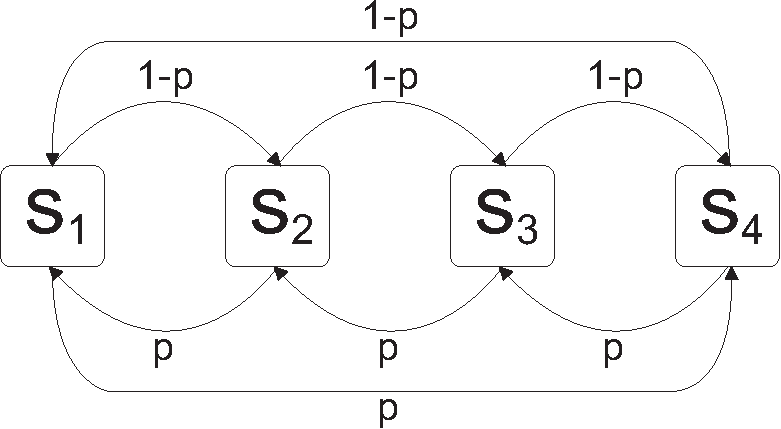
\includegraphics[width=0.4\columnwidth]{Grafiken/Uebergangsgraph}
\end{center}
Eine Verteilung heißt \textbf{stationär}, wenn gilt:
\[\overrightarrow{p}_{\infty}=\mathbf{\Pi}\overrightarrow{p}_{\infty}\]

\section{Zufallsprozesse}
\textbf{Reeller Zufallsprozess:} $\mathsf{X}_{t} : \Omega \mapsto \mathbb{R}, \ t \in \mathbb{R}$\\
$\Rightarrow$ Zufallsfolge ist ein diskreter Zufallsprozess

\subsection{Ensemble und Musterfunktion}
Möglichkeiten der Interpretation eines Zufallsprozesses:
\begin{abc}
\item als \textbf{Ensemble} einer nicht abzählbaren Menge von Zufallsvariablen $X_{t}$ mit $t \in \mathbb{R}$
\item \textbf{Schar von Musterfunktionen} $\mathsf{X}_{t}(\omega) : \mathbb{R} \mapsto \mathbb{R}, \ t \mapsto \mathsf{X}_{t}(\omega)$ als deterministische Funktion von $t$ mit einem gegebenen Ereignis $\omega \in \Omega$
\end{abc}

\subsection{Verteilungen und Momente}
\begin{abc}
\item \textbf{Erwartungswertfunktion} \[  \quad \mu_{\mathsf{X}}(t) = \erw[\mathsf{X}_{t}] \]
\item \textbf{Autokorrelationsfunktion} \[ \quad r_{\mathsf{X}}(s,t) = \erw[\mathsf{X}_{s} \mathsf{X}_{t}]=r_{\mathsf{X}}(t,s) \]
\item \textbf{Autokovarianzfunktion}  \[ c_{\mathsf{X}}(s,t) = \cov(\mathsf{X}_{s}, \mathsf{X}_{t}) =  r_{\mathsf{X}}(s,t) - \mu_{\mathsf{X}}(s) \mu_{\mathsf{X}}(t) \]
\end{abc}

\subsection{Wiener-Prozess (ist \textbf{kein} Zählprozess!)}
Addition/Subtraktion eines zufälligen Wertes je infinitesimalem Zeitintervall.  \\
Der Zufallsprozess $(\mathsf{S}_{t} : t \in \mathbb{R}_{+})$ mit  $\mathsf{S}_{t} \sim \mathcal{N} (0, \sigma^{2} t)$ heißt \textbf{Wiener-Prozess}.
\begin{align}
S_n&=[S_t]_{t=nT};\;\;\;\;n\rightarrow\infty,T\rightarrow 0\nonumber\\
\left[\erw[\mathsf{S}_{t}]\right]_{t=nT} & = \erw[\mathsf{S}_{n}] = 0 \nonumber \\
\left[\var[\mathsf{S}_{t}]\right]_{t=nT} & = \var[\mathsf{S}_{n}] = n \delta^{2} = \left\lfloor \frac{t}{T} \right\rfloor \delta^{2}=\sigma^2t \ \text{mit} \ \delta = \sqrt{\sigma^{2}T} \nonumber
\end{align}
Die Varianz der Normalverteilung ist hier also zeitabhängig:
\[ f_{\mathsf{S}_{t}}(x) = \frac{1}{\sqrt{2\pi \sigma^{2} t}} \operatorname{exp}\left(-\frac{x^{2}}{2\sigma^{2}t} \right) , \quad t \in \mathbb{R}_{+}\]
\subsubsection{Eigenschaften des Wiener-Prozesses}
Sei  ($\mathsf{W}_{t} : t \in \mathbb{R}_{+}$) mit $\sigma > 0$ ein Wiener-Prozess, dann gilt:
\begin{abc}
\item $P(\{\mathsf{W}_{0} = 0 \}) = 1$ (Wiener-Prozess startet stets im Koordinatenursprung)
\item ($\mathsf{W}_{t} : t \in \mathbb{R}_{+}$) hat unabhängige Inkremente
\item $\mathsf{W}_{t} - \mathsf{W}_{s} \sim \mathcal{N} (0, \sigma^{2}(t-s)) \ \forall 0 \leq s \leq t$
\item $\mathsf{W}_{t}(\omega)$ ist stetige Musterfunktion mit Wahrscheinlichkeit 1
\item \textbf{Erwartungswertfunktion}
\[ \mu_{\mathsf{W}}(t) = \erw[\mathsf{W}_{t}] = \erw[\mathsf{W}_{t} - \mathsf{W}_{0}] = 0\]
\item \textbf{Autokorrelationsfunktion}
\[r_{\mathsf{W}}(s,t) = c_{\mathsf{W}}(s,t) = \sigma^{2} \operatorname{min}\{s,t\} \]
\end{abc}

\subsection{Poisson-Prozess (\textbf{Zählprozess}, $\mathsf{N}_{t} : t \in \mathbb{R}_{+})$}
Das Zeitintervall bis zur nächsten Inkrementierung ist immer identisch exponentialverteilt.\\
Die Inkremente der ZV $\mathsf{X}_t-\mathsf{X}_s$ sind Poisson-verteilt:
\[p_{\mathsf{X}_t-\mathsf{Y}_t}(n)=e^{-\lambda_\mathsf{X}(t-s)}\frac{[\lambda_\mathsf{X}(t-s)]^n}{n!};\;\;\;n\in\mathbb{N}_0\]
\textbf{Konstruktion}
\[ \mathsf{N}_{t} = \sum \limits_{i = 1}^{\infty} u(t - \mathsf{T}_{i}), \quad T_{i} = \sum \limits_{j=1}^{i} \mathsf{X}_{j}\]
\textbf{Wahrscheinlichkeitsdichtefunktion}
\[ f_{\mathsf{T}_{i}}(t) = \frac{\lambda^{i}}{(i-1)!} t^{i-1}\operatorname{e}^{-\lambda t}, \quad t \geq 0\]
Wahrscheinlichkeit, dass bis zum Zeitpunkt $t$ genau $n$ zufällige Inkrementierungen stattgefunden haben:
\[ P(\{\mathsf{N}_{t} = n \}) = \frac{(\lambda t)^{n}}{n!} \operatorname{e}^{-\lambda t} \quad n \in \mathbb{N}, t \in \mathbb{R}_{+}\]

\subsubsection{Eigenschaften des Poisson-Prozesses}
\begin{abc}
\item \textbf{Erwartungswertfunktion}
\[ \mu_{\mathsf{N}}(t) = \erw[\mathsf{N}_{t}] = \erw[\mathsf{N}_{t} - \mathsf{N}_{0}] = \lambda t\]
\item \textbf{Autokorrelationsfunktion}
\[ r_{\mathsf{N}}(t_1,t_2)=\erw[N_{t_1}N_{t_2}] = \lambda \operatorname{min}\{t_1,t_2\} + \lambda^{2} t_1t_2\]
\item \textbf{Autokovarianzfolge}
\begin{equation*}
\begin{split}
c_{\mathsf{N}}(t_1,t_2) &= \text{Cov}[N_{t_1},N_{t_2}]=r_N(t_1,t_2)-\mu_N(t_1)\mu_N(t_2)\\
&= \lambda \operatorname{min}\{t_1,t_2\}
\end{split}
\end{equation*}
\item Musterfunktion des $\sim$ ist Zählfunktion\\
($f(0) = 0, f$ monoton steigend $\Rightarrow \mathsf{N}_{t2} \geq \mathsf{N}_{t1}$ gilt immer!)
\end{abc}

\subsection{Klassifikation reeller Zufallsprozesse}
\subsubsection*{Eigenschaften eines einzelnen Zufallsprozesses} 
\begin{iii}
\item \textbf{Stationarität} eines ZP
\begin{align} F_{\mathsf{X}_{t_{1}},\dots,\mathsf{X}_{t_{n}}} (x_{1}, \dots x_{n}) = F_{\mathsf{X}_{t_{1}+s},\dots,\mathsf{X}_{t_{n}+s}} (x_{1}, \dots x_{n})  \nonumber \\
 \forall \begin{bmatrix}x_{1}, \dots, x_{n} \end{bmatrix}^{T} \in \mathbb{R}^{n}, \begin{bmatrix}t_{1}, \dots, t_{n} \end{bmatrix}^{T} \in \mathbb{R}^{n}, s \in \mathbb{R}, n \in \mathbb{R}  \nonumber
\end{align}
\item \textbf{Stationarität im weiteren Sinne (WSS)}
\begin{align}
  \mu_{\mathsf{X}}(t) &= \mu_{\mathsf{X}}(t+s);\;\;\;\; \forall t,s \in \mathbb{R} \nonumber \\
  r_{\mathsf{X}}(t_1,t_2) &= r_{\mathsf{X}}(t_1 + s, t_2 + s)=r_{\mathsf{X}}(\underbrace{t_1-t_2}_{\tau})=r_{\mathsf{X}}(-\tau) \nonumber
\end{align}
Stationarität $\Rightarrow$ Stationarität im weiteren Sinne (Umkehrung gilt nicht!).
\item \textbf{Zyklische WSS}
Für periodische $ \mu_{\mathsf{X}}(t)$ und $ r_{\mathsf{X}}(t_1,t_2)$ mit $T > 0$ gilt:
\begin{align}
  \mu_{\mathsf{X}}(t) &= \mu_{\mathsf{X}}(t+T) & \forall t \in \mathbb{R} \nonumber \\
  r_{\mathsf{X}}(t_1,t_2) &= r_{\mathsf{X}}(t_1 + T, t_2 + T) & \forall t_1,t_2 \in \mathbb{R} \nonumber
\end{align}
aus WSS $\Rightarrow$ zyklische WSS
\end{iii}

\subsubsection*{Eigenschaften von zwei Zufallsprozessen} 
Seien $(\mathsf{X}_{t}: t \in \mathbb{R})$ und $(\mathsf{Y}_{t}: t \in \mathbb{R})$ zwei ZP auf demselben Wahrscheinlichkeitsraum
\begin{iii}
\item \textbf{Gemeinsame Stationarität} \\ $\mathsf{X}_{t}$ und $\mathsf{Y}_{t}$ sind zwei reelle jeweils selbst stationäre ZP und ihre gemeinsamen Verteilungen verschiebungsinvariant.
\item \textbf{Kreuzkorrelationsfunktion}
\[ r_{\mathsf{X,Y}}(s,t) = \erw[\mathsf{X}_{s} \mathsf{Y}_{t}] = r_{\mathsf{Y,X}}(t,s) \]
\item \textbf{Kreuzkovarianzfunktion}
\[ c_{\mathsf{X,Y}}(s,t) =r_{\mathsf{X,Y}}(s,t) - \mu_{\mathsf{X}}(s) \mu_{\mathsf{Y}}(t) = c_{\mathsf{Y,X}}(t,s) \]
\item \textbf{Gemeinsame Stationarität im weiteren Sinne} \\$\mathsf{X}_{t}$ und $\mathsf{Y}_{t}$ sind zwei reelle jeweils selbst im weiteren Sinne stationäre ZP und es gilt
\[ r_{\mathsf{X,Y}}(t_1,t_2) = r_{\mathsf{X,Y}}(t_1+s,t_2+s) \quad \forall t_1,t_2,s \in \mathbb{R}\]
\item \textbf{Stochastische Unabhängigkeit}
\begin{equation*}
\begin{split}
&F_{\mathsf{X}_{t_1},...,\mathsf{X}_{t_n},\mathsf{Y}_{t_{n+1}},...,\mathsf{Y}_{t_{n+m}}}(x_1,...,x_n,y_1,...,y_m)\\
=&F_{\mathsf{X}_{t_1},...,\mathsf{X}_{t_n}}(x_1,...,x_n)F_{\mathsf{Y}_{t_{n+1}},...,\mathsf{Y}_{t_{n+m}}}(y_1,...,y_m)
\end{split}
\end{equation*}
\item \textbf{Stochastische Unkorreliertheit} 
\[ c_{\mathsf{X,Y}}(s,t) = 0 \Leftrightarrow r_{\mathsf{X,Y}}(s,t) = \mu_{\mathsf{X}}(s) \mu_{\mathsf{Y}}(t) \quad \forall s,t \in \mathbb{R} \]
\item \textbf{Stochastische Orthogonalität}
\[ r_{\mathsf{X,Y}}(s,t) = 0 \quad \forall s, t \in \mathbb{R}\]
\end{iii}

\subsection{Eigenschaften der Auto- und Kreuzkorrelationsfunktion von gemeinsam WSS Zufallsprozessen}
\begin{align}
r_{\mathsf{X}}(\tau) & \leq r_{\mathsf{X}}(0) \nonumber \\
|r_{\mathsf{X,Y}}(\tau)| & \leq \sqrt{r_{\mathsf{X}}(0) r_{\mathsf{Y}}(0)} \nonumber \\
r_{\mathsf{X}}(\tau) & = r_{\mathsf{X}}(- \tau) \ \text{(AKF gerade, achsensymm.)} \nonumber \\
\mathbf{a}^{T}\mathbf{R}_{\mathsf{X}}\mathbf{a} & \geq 0 \nonumber \\
 [ \mathbf{R}_{\mathsf{X}} ]_{k,l} & = r_{\mathsf{X}}(t_{k}-t_{l}) \quad \forall t_{k},t_{l} \in \mathbb{R}, \mathbf{a} \in \mathbb{R}^{n} \nonumber
\end{align}

\subsection{Leistungsdichtespektrum reeller WSS Zufallsprozesse}
$\rightarrow$ existiert nur für WSS Zufallsprozesse!
\[ S_{\mathsf{X}}(f) = \int \limits_{- \infty}^{\infty} r_{\mathsf{X}}(\tau) \operatorname{e}^{-j 2 \pi f \tau} \, d\tau \]
(Wiener-Chintschin-Theorem)\\\\
\textbf{Eigenschaften}
\begin{align}
S_{\mathsf{X}}(f) &= S_{\mathsf{X}}^{*}(f) & \forall f \in \mathbb{R} \nonumber \\
S_{\mathsf{X}}(f) &= S_{\mathsf{X}}(-f) & \forall f \in \mathbb{R} \nonumber \\
 \int \limits_{- \infty}^{\infty} S_{\mathsf{X}}(f) \, df & = r_{\mathsf{X}}(0) = \sigma_{\mathsf{X}}^{2} + \mu_{\mathsf{X}}^{2}=\erw[\mathsf{X}^2] \nonumber \\
S_{\mathsf{X}}(f) & \geq 0 & \forall f \in \mathbb{R} \nonumber
\end{align}

\section{Zufallsprozesse und lineare Systeme}
\subsection{Lineare zeitinvariante Systeme}
Beschreibung eines LTI-Systems durch \textbf{Impulsantwort}:
\begin{align}
y(t) & =  (h \ast x)(t) = \int_{- \infty}^{\infty} h(t - \tau) x(\tau) \, d\tau \nonumber = \int_{- \infty}^{\infty} h(\tau) x(t- \tau) \, d\tau \nonumber
\end{align}
Im Frequenzraum gilt dann folglich:
\[ Y(f) =  H(f)X(f) \]

\subsection{Erwartungswert- und Korrelationsfunktionen}
Ausgang eines mit dem Zufallsprozess $\mathsf{X}_{t}$ beaufschlagten linearen Systems ist wieder ein Zufallsprozess:
\begin{align}
\mathsf{Y}_{t} & = \int_{- \infty}^{\infty} h(t-\tau) \mathsf{X}_{\tau} \, dt = \int_{- \infty}^{\infty} h(\tau) \mathsf{X}_{t-\tau} \, dt \nonumber
\end{align}
Bei Filterung eines WSS Zufallsprozesses $\mathsf{X}_{t}$ mit einem LTI-System sind $\mathsf{X}_{t}$ und der gefilterte Zufallsprozess $\mathsf{Y}_{t}$ gemeinsam \textbf{WSS}. Dann gilt:
\begin{iii}
\item \textbf{Erwartungswertfunktion}
\[ \mu_{\mathsf{Y}} = \mu_{\mathsf{X}} \int_{- \infty}^{\infty} h(t) \, dt \]
\item \textbf{Kreuzkorrelationsfunktion}
\begin{equation*}
\begin{split}
r_{\mathsf{Y,X}}(\tau) &= (h\ast r_{\mathsf{X,X}})(\tau)=(h \ast r_{\mathsf{X}})(\tau) \quad\\
r_{\mathsf{X,Y}}(\tau)&=(h\ast r_{\mathsf{X}})(-\tau)=(\tilde{h}*r_{\mathsf{X}})(\tau)
\end{split}
\end{equation*}
\item \textbf{Autokorrelationsfunktion}
\[ r_{\mathsf{Y}}(\tau) = (\tilde{h} \ast h \ast r_{\mathsf{X}})(\tau) \quad \text{mit} \ \tilde{h}(\tau) = h(- \tau) \]
\end{iii}

\subsection{Leistungsdichtespektren}
Leistungsdichtespektrum ist die Fourier-Transformierte der entsprechenden Korrelationsfunktion, folglich gilt:
\begin{align}
r_{\mathsf{Y}}(\tau) & \fa S_{\mathsf{Y}}(f) \nonumber \\
r_{\mathsf{Y,X}}(\tau) & \fa S_{\mathsf{Y},\mathsf{X}}(f) \nonumber\\
r_{\mathsf{Y,X}}(-\tau) & \fa S^{*}_{\mathsf{Y},\mathsf{X}}(f) \nonumber
\end{align}

Leistungsdichtespektrum der
\begin{iii}
\item \textbf{Autokorrelationsfunktion}
\[ S_{\mathsf{Y}}(f) = |H(f)|^{2} S_{\mathsf{X}}(f)\]
\item \textbf{Kreuzkorrelationsfunktion}
\begin{align}
S_{\mathsf{Y,X}}(f) & = H(f) S_{\mathsf{X}}(f) \nonumber \\
S_{\mathsf{X,Y}}(f) & = H^{*}(f) S_{\mathsf{X}}(f) \nonumber 
\end{align}
\end{iii}
\vspace{1cm}
Diese Formelsammlung ist eine überarbeitete und erweiterte Version der ''Stochastische Signale Formelsammlung'' von Tobias Grabmeier (Originalversion 2011-07-02), Sebastian Krosche (Version 2012-02-09), Johannes Pickart (Version 2013-02-13).\\\\
Lizenz: CC BY-NC-SA 3.0\\
\url{http://creativecommons.org/licenses/by-nc-sa/3.0/de/}

\end{document}
